\chapter{Basic Algorithms}

I will now talk about two very common machine learning algorithms, the boosted decision tree (BDT) and the neural net. Neural nets in particular form the basis of most modern machine learning, and all advanced architectures discussed in this thesis will be some form of neural network.

\section{BDTs}

Simply speaking, a decision tree is simply a series of branching paths based on input data, which one can follow to reach a conclusion. An example of a very simple decision tree is shown in Figure~\ref{decision_tree}. Decision trees are similar to how objects and signal regions are selected in a traditional high-energy-physics analysis. For example, one may ask whether an event has more than, less than, or equal to three leptons. If the event has exactly three leptons, one may ask whether the top two leptons have dilepton mass within a certain range, etc. Based on these decisions, an experimenter can decide what signal region an event belongs in. As another example, imagine that we are trying to determine what kind of particle we have seen in an event. We could ask whether the particle left a track in the inner detector, whether the amount of energy it deposited in the calorimeter is in a certain range, etc. Given a random ordered set of input variables, an optimal decision tree can be calculated for decisions made in that specific order.

A boosted decision tree is created by combining many different decision trees together \cite{BDT}. Any given decision tree can be very weak, containing only a small number of branches and a small maximum depth. However, by taking the weighted results of many decision trees together, we can get a more accurate result than can be achieved by any single tree. For the sake of space, the AdaBoost BDT training algorithm will not be discussed here.

\begin{figure}[t]
    \centering
    %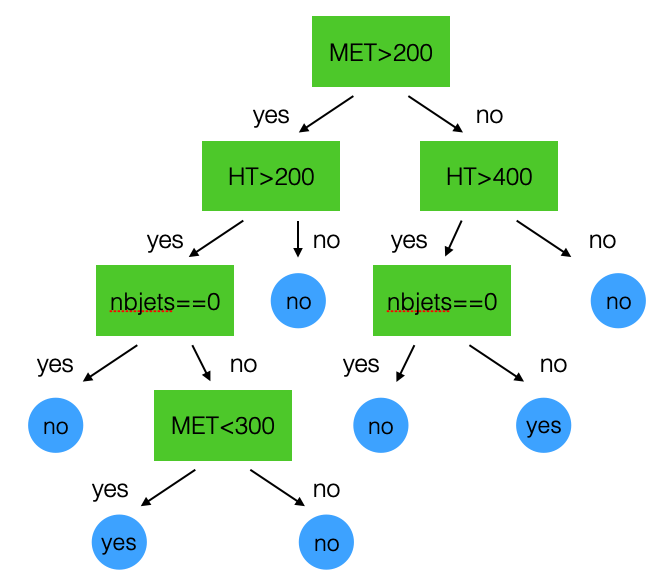
\includegraphics[width=0.5\linewidth]{images/decision_tree.png}
    \caption{An example of a decision tree that a child may use to classify a household pet.}
    \label{decision_tree}
\end{figure}

\section{Neural Nets}

A neural net is a machine learning architecture based on the physical structure of neurons in the human brain \cite{neural_net}. The basic unit of a neural net is a neuron, which has a numerical value, one or more inputs, and one or more outputs. These neurons are connected together so that the output of one neuron becomes the input of one or more other neurons. Here we will only consider simple feed-forward neural nets, where all the inputs to a neuron come from neurons closer to the beginning of the net, and all the outputs of that neuron go to neurons nearer the end of the net. That is, there are no "loops", and there are no connections between neurons at the same depth. The input values for an event form the first layer of neurons, and the output is derived from the last layer. Each link between neurons is associated with a "weight", or multiplicative constant. Each neuron is also associated with a "bias", or an additive constant. Letting $y_i$ be the value of the $i^{th}$ neuron, $w_{i,j}$ be the value of the weight between neurons $i$ and $j$, and $b_i$ be the bias associated with neuron $i$, we see that the value of a neuron is equal to $y_j = \sum{w_{i,j}y_i} + b_j$. Each neuron is also typically followed by a nonlinear "activation" function, so that the result of the entire net is not simply equivalent to a single matrix operation on the input. We see then that for a given set of weights and biases, we can calculate the output value for a net given any inputs.

In order to train a neural net, we use "back-propagation", meaning that for each event (or set of events) we perform gradient descent on each weight and bias in order to minimize the resulting loss function. Over the course of many events, the net can fall into a state where it produces the correct outputs with high accuracy. In this way, the neural net training is simply a form of function optimization. Many important topics, such as how to weight initialization, methods of gradient descent, net architectures, etc. will not be discussed in this paper.

\begin{figure}[t]
    \centering
    %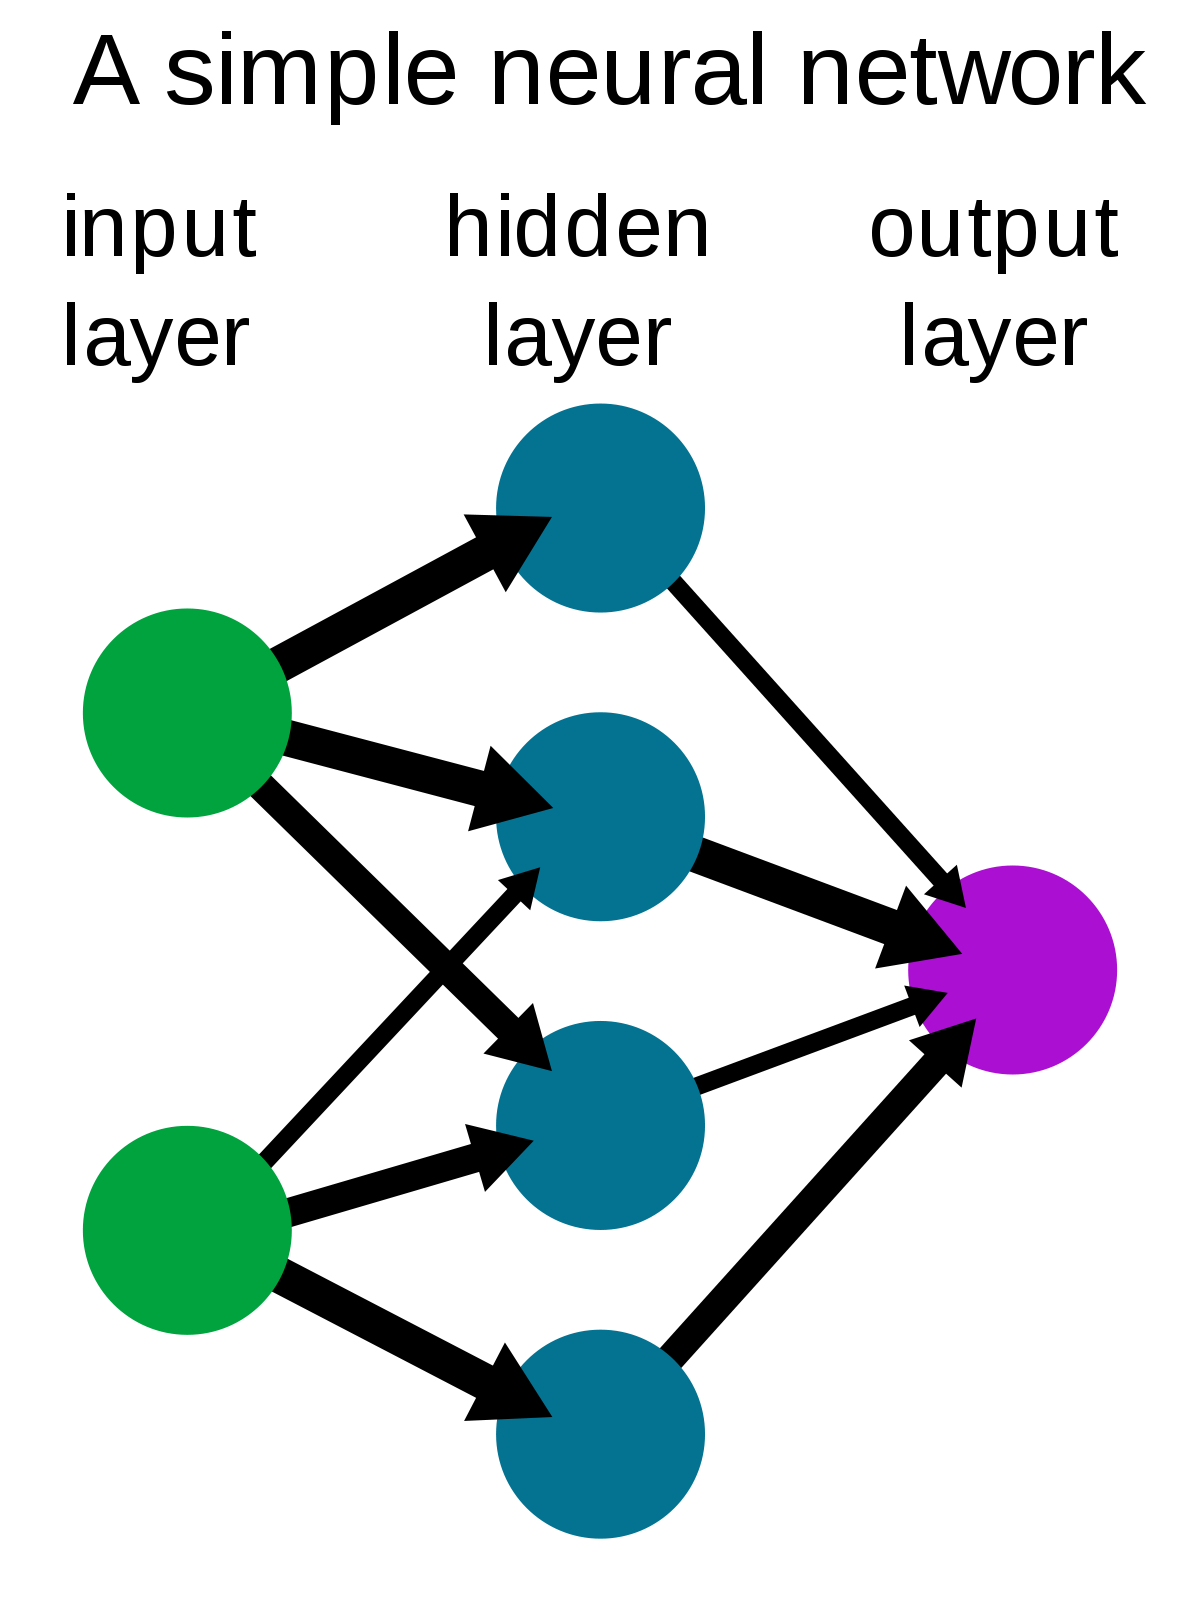
\includegraphics[width=0.5\linewidth]{images/neural_net.png}
    \caption{A diagram showing a typical densely-connected neural net.}
    \label{neural_net}
\end{figure}

\section{Basic Training Concepts}

\subsection*{Activation Functions}

\subsection*{Overfitting, Underfitting, and Regularization}

\subsection*{Dropout Layers}

\subsection*{Batch Normalization}

\subsection*{Hyperparameter Optimization}